
% !TEX root = DesignDocument.tex

\chapter{The Data Encryption Standard}

In 1975 the National Bureau of Standards along with IBM and the National Security Agency released the first nationally standardized encryption algorithm.
This algorithm at the time called LUCIFER and eventually labed DES was the national standard for 25 years until it was supplanted by the Advanced Encryption Standard in 2000.
DES still has historic and scolastic significance which is why two implemenations of it are provided here.
The first is a simplified version and the second is a Full software implementation of DES.

\begin{figure}[ht]
\begin{center}
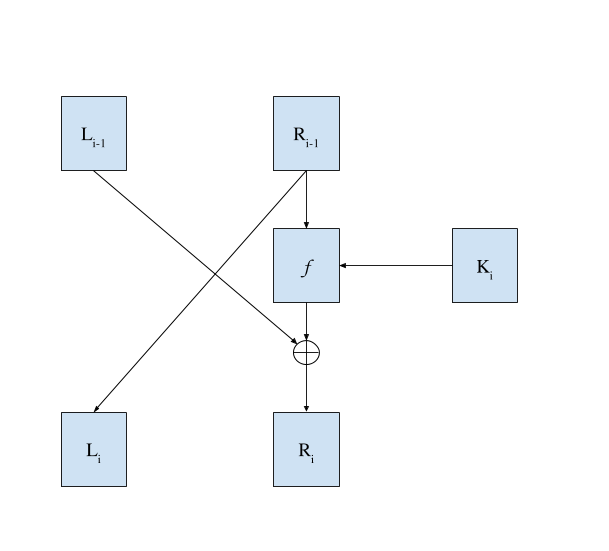
\includegraphics[width=0.75\textwidth]{./feistel}
\end{center}
\caption{Feistel system structure.}
\end{figure}

DES is a block cipher and a Feistel system. 
Named after Horst Feistel who was on the team which created LUCIFER.
Feistel systems tend to have many similiar structures to them.
These include bit permutations, Multiple XORs and Substitution boxes.
The intent of any Feistel system is to create large changes in the plaintext with ever round.
However often as a consquence of their structure, encryption and decryption schemes are nearly identical.


\section{Simplified DES (SDES) }

The simplified version of the Data encryption standard ( SDES ) that is presented here uses four rounds and two substitution boxes to encrypt plaintext.
It is a block cypher just like DES, but instead of 64-bit block it uses 12-bit blocks. 
The key is also much smaller only 9-bits ( Although only 8-bits are used every round).

\subsection{Encryption and Decryption}

\begin{figure}[ht]
\begin{center}
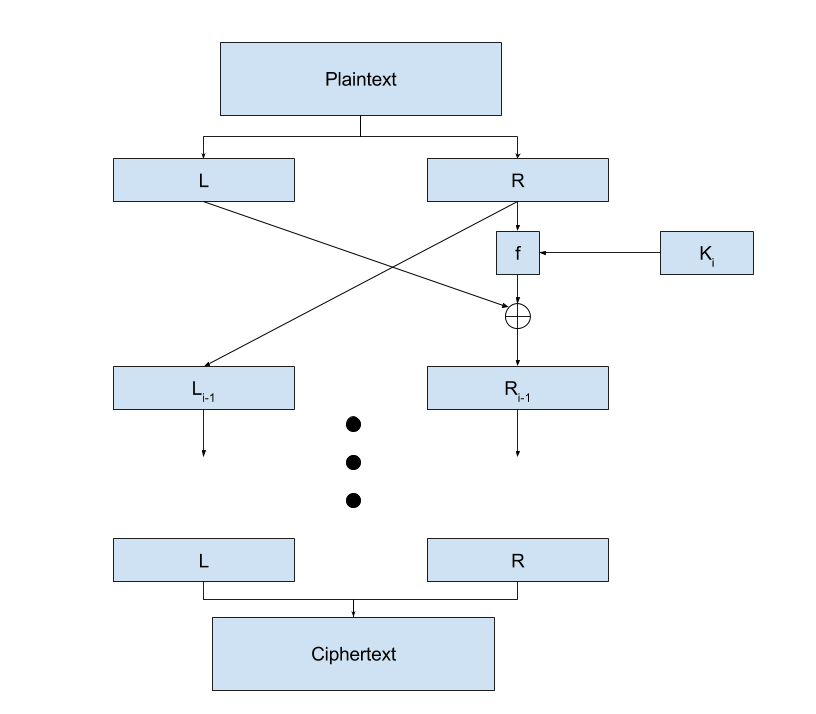
\includegraphics[width=0.75\textwidth]{./SDESflow}
\end{center}
\caption{Feistel system structure.}
\end{figure}

\begin{figure}[ht]
\begin{center}
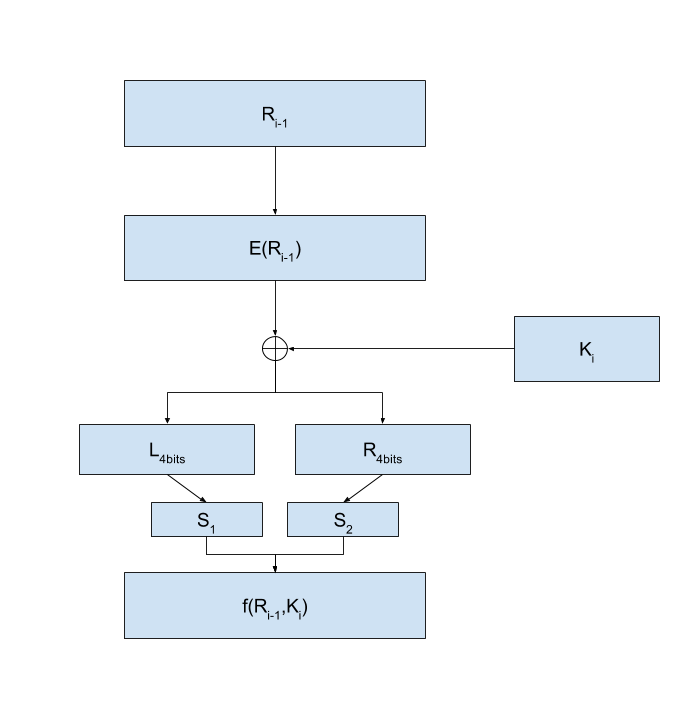
\includegraphics[width=0.5\textwidth]{./fFunc}
\end{center}
\caption{ One round of the SDES Feisel System.}
\end{figure}



\section{64-bit DES}

\begin{figure}[ht]
\begin{center}
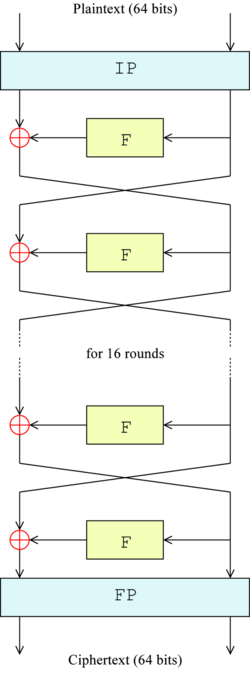
\includegraphics[width=0.5\textwidth]{./DESAlgo}
\end{center}
\caption{DES Algorithm Overview}
\end{figure}

\begin{figure}[ht]
\begin{center}
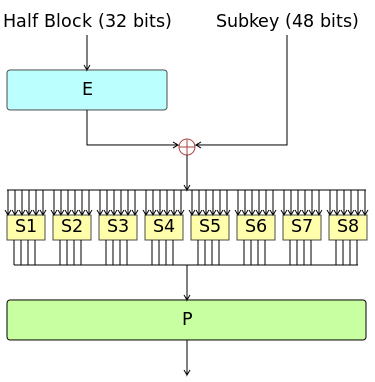
\includegraphics[width=0.4\textwidth]{./FFfunc}
\end{center}
\caption{DES Function $f(R_{i-1},K_i)$}
\end{figure}

\begin{figure}[ht]
\begin{center}
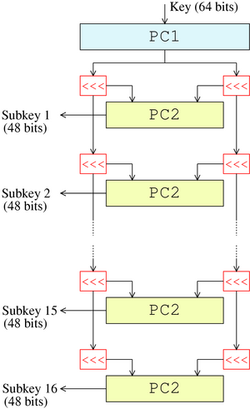
\includegraphics[width=0.3\textwidth]{./DESkey}
\end{center}
\caption{DES's key scheduler}
\end{figure}

\subsection{Encryption}
\subsection{Decryption}
